%============= Disclaimer ======================
% This template has been modified by LeninGF from
% a previous thesis template in overleaf to address
% the font and style of EPN, 
% hope it helps and may science be with U
%============= Disclaimer ======================
\documentclass[12pt,oneside]{report}  %twoside
\usepackage[utf8]{inputenc}
\usepackage{graphicx}
% \graphicspath{ {images/} }
\usepackage{caption}
\usepackage{subcaption}
\usepackage{blindtext}  % to fill with randomtext
% \usepackage[a4paper,width=150mm,top=30mm,bottom=25mm,bindingoffset=6mm]{geometry}
\usepackage[a4paper,tmargin=3cm,bmargin=2.5cm,lmargin=3cm, rmargin=2.5cm, bindingoffset=6mm]{geometry}
\usepackage{fancyhdr}
\pagestyle{fancy}
\fancyhead{}
\fancyhead[RO,LE]{Transfer and ensemble learning models in breast mammogram pathology classification}
\fancyfoot{}
\fancyfoot[LE,RO]{\thepage}
\fancyfoot[LO,CE]{Chapter \thechapter}
\fancyfoot[CO,RE]{Lenin G. Falconí}
\renewcommand{\headrulewidth}{0.4pt}
\renewcommand{\footrulewidth}{0.4pt}

%======== number format ===============
\usepackage{numprint}
%========BIBLIOGRAPHY==================
% \usepackage[backend=biber, style=authoryear-ibid, citestyle=apa, sorting=anyt, maxcitenames=2]{biblatex}   % orden alfabeitco o nty
\usepackage[backend=biber,style=apa,babel=other,maxcitenames=3]{biblatex}
\addbibresource{mendeley.bib}
%========LUALATEX======================
% Usar LuaLatex para compilar
% Tipo de Letra cambio para xelatex
\usepackage{fontspec}
\setmainfont{Arial}

% Arial
% \setsansfont[
% BoldFont=fonts/arialbd.ttf,
% ItalicFont=fonts/ariali.ttf,
% BoldItalicFont=fonts/arialbi.ttf
% ]{fonts/arial.ttf}
%========XELATEX======================
%========PDFLATEX======================

% \usepackage[T1]{fontenc}
% \usepackage{helvet}
%========PDFLATEX======================

\usepackage{anyfontsize}
% para hacer comillas de copia textual
\usepackage{dirtytalk}

% para hiperlinks
\usepackage{hyperref}
% for boxes around text
\usepackage{tcolorbox}
% to strike through text
\usepackage{ulem}
% to have tabularx 
\usepackage{tabularx}
% to have tabu tables
\usepackage{tabu}
\usepackage{booktabs}

% to use csv files
\usepackage{siunitx}
\usepackage{pgfplotstable}
\usepackage{booktabs}

% Definition styles:
\usepackage{amsthm}
\theoremstyle{definition}
\newtheorem{definition}{Definition}[section]

% Math Styles
\usepackage{amsmath, amssymb, amsfonts}
\usepackage{mathrsfs}
% Increase of math font size 
\usepackage{relsize}
\DeclareMathOperator{\ypred}{\phi}  %options \hslash

% Lorem Ipsum 
\usepackage{lipsum}
%========= Defining Values of the Thesis=============%
\newcommand{\ThesisTitle}{\MakeUppercase{Thesis Title} }
\newcommand{\AuthorName}{Philip J. Fry}
\newcommand{\AuthorLongName}{Philp Jay Fry }
\newcommand{\CoodirectorName}{Carl Edward Sagan}
\newcommand{\DirectorName}{Augusta Ada Byron Lovelace}
\title{\ThesisTitle}
\author{\AuthorName}
\date{Day Month Year}
%======== Controlling numeration ===================%
% https://tex.stackexchange.com/questions/154646/is-there-an-easy-way-to-get-the-frontmatter-mainmatter-and-backmatter-in-a-l
% http://www-users.york.ac.uk/~pjh503/LaTeX/frontstuff.html
\newcommand\frontmatter{%
    \cleardoublepage
  %\@mainmatterfalse
  \pagenumbering{roman}}

\newcommand\mainmatter{%
    \cleardoublepage
 % \@mainmattertrue
  \pagenumbering{arabic}}

%======== Controling Line Spacing =================% 
% espacio de 1.5 como en dummy word
\linespread{1.3}


\begin{document}

\begin{titlepage}
    \begin{center}
    % * AFTER VSPACE FORECE TO BE EXECUTED
        % \vspace*{\baselineskip}
        \vspace*{0.5\baselineskip}
        
        
        % \textbf{\LARGE{ESCUELA POLITÉCNICA NACIONAL}}
        \textbf{{\fontsize{2em}{2em} \selectfont ESCUELA POLITÉCNICA NACIONAL}}
        
        \vspace*{0.5\baselineskip}
        \vspace*{\baselineskip}
        \large{\textbf{FACULTAD DE SISTEMAS}}\\
        % \textbf{{\fontsize{1.4em}{1.4em} \selectfont FACULTAD DE SISTEMAS}}
        
        \vspace*{\baselineskip}
        
        \large{\textbf{UNIDAD DE TITULACIÓN}}\\
        
        \vspace*{\baselineskip}
        \vspace*{\baselineskip}
        
        \large{\textbf{\textsc{A thesis interesting name}}}\\
        
        % \vspace*{\baselineskip}
        \vspace*{\baselineskip}
        \vspace*{\baselineskip}
        \vspace*{0.5\baselineskip}
        
        \textbf{\normalsize{TRABAJO DE TITULACIÓN PREVIO A LA OBTENCIÓN DEL GRADO DE MAGÍSTER EN COMPUTACIÓN}}\\
        
        \vspace*{\baselineskip}
        \vspace*{\baselineskip}
        \vspace*{0.5\baselineskip}
        
        \textbf{\normalsize{PHILIP JAY FRY}}\\
        \textbf{\normalsize{philip.fry@epn.edu.ec}}\\
        
        \vspace*{\baselineskip}
        \vspace*{\baselineskip}
        
        \textbf{\normalsize{Director: AUGUSTA ADA BYRON LOVELACE}}\\
        \textbf{\normalsize{ada.lovelace@epn.edu.ec}}\\
        
        \vspace*{\baselineskip}
        % \vspace*{\baselineskip}
        
        \textbf{\normalsize{Co-Director: HUBERT JAY FARNSWORTH}}\\
        \textbf{\normalsize{hubbyj.farnsworth@epn.edu.ec}}\\
        
        
        \vspace*{\baselineskip}
        \vspace*{\baselineskip}
        \normalsize{\textbf{2019}}
        
    \end{center}
\end{titlepage}
\thispagestyle{empty}
    \vspace*{1em}
    \vspace*{1em}
    \begin{center}
        \textbf{\large{DIRECTOR'S APPROVAL}}
    \end{center}
    \vspace*{1em}
    \vspace*{1em}
    \setlength{\parindent}{0em}
    As director of the \ThesisTitle degree work developed by \AuthorName, student of the Master's degree in Computing, having supervised the completion of this work and made the corresponding corrections, I approve the final drafting of the written document to continue with the corresponding procedures to support oral defense.\\
    \vspace*{1em}
    \vspace*{1em}
    \vspace*{1em}
    \vspace*{1em}
    
    \begin{center}
        \begin{tabular}{c c c}
        \hfill  & \rule{8cm}{0.4pt} & \hfill \\
        \hfill  & \textbf{\DirectorName} & \hfill \\
        \hfill  & \textbf{DIRECTOR} & \hfill \\
        
        \end{tabular}
    \end{center}
    % \begin{center}
    %     \begin{tabular}{@{}p{.5in}p{4in}@{}}
    
    %      & \hrulefill \\
    %      & Fats Domino, Ph.D.\\
    %      & Chair of the Department of Nutrition\\
        
    % \end{tabular}    
    % \end{center}
    
\newpage





\thispagestyle{empty}
    \vspace*{1em}
    \vspace*{1em}
    \begin{center}
        \textbf{\large{CO-DIRECTOR'S APPROVAL}}
    \end{center}
    \vspace*{1em}
    \vspace*{1em}
    \setlength{\parindent}{0em}
    As co-director of the \ThesisTitle degree work developed by \AuthorName, student of the Master's degree in Computing, having supervised the completion of this work and made the corresponding corrections, I approve the final drafting of the written document to continue with the corresponding procedures to support oral defense.\\
    \vspace*{1em}
    \vspace*{1em}
    \vspace*{1em}
    \vspace*{1em}
    
    \begin{center}
        \begin{tabular}{c c c}
        \hfill  & \rule{8cm}{0.4pt} & \hfill \\
        \hfill  & \textbf{\CoodirectorName} & \hfill \\
        \hfill  & \textbf{CO-DIRECTOR} & \hfill \\
        
        \end{tabular}
    \end{center}
    % \begin{center}
    %     \begin{tabular}{@{}p{.5in}p{4in}@{}}
    
    %      & \hrulefill \\
    %      & Fats Domino, Ph.D.\\
    %      & Chair of the Department of Nutrition\\
        
    % \end{tabular}    
    % \end{center}
    
\newpage





\thispagestyle{empty}
    \vspace*{1em}
    \vspace*{1em}
    \begin{center}
        \textbf{\large{AUTHORSHIP DECLARATION}}
    \end{center}
    \vspace*{1em}
    \vspace*{1em}
    \setlength{\parindent}{0em}
    I, \AuthorLongName, declare under oath that the work described here is my responsibility; that has not been previously submitted for any degree or professional qualification; and, that I have consulted the bibliographic references included in this document.\\
    Escuela Politécnica Nacional (EPN) and the participating universities in the project XXXX may use the rights corresponding to this work, as established by the Intellectual Property Law, by its Regulations and by current institutional regulations.\\
    \vspace*{1em}
    \vspace*{1em}
    \vspace*{1em}
    \vspace*{1em}
    
    \begin{center}
        \begin{tabular}{c c c}
        \hfill  & \rule{8cm}{0.4pt} & \hfill \\
        % \hfill  & \textbf{\AuthorName} & \hfill \\
        \hfill  & \textbf{\AuthorLongName} & \hfill \\
        % \hfill  & \textbf{DIRECTOR} & \hfill \\
        
        \end{tabular}
    \end{center}
    % \begin{center}
    %     \begin{tabular}{@{}p{.5in}p{4in}@{}}
    
    %      & \hrulefill \\
    %      & Fats Domino, Ph.D.\\
    %      & Chair of the Department of Nutrition\\
        
    % \end{tabular}    
    % \end{center}
    
\newpage





\thispagestyle{empty}
    \vspace*{1em}
    \vspace*{1em}
    \vspace*{1em}
    \vspace*{1em}
    \begin{center}
        \textbf{\large{DEDICATED TO}}
    \end{center}
    \vspace*{1em}
    \vspace*{1em}
    \setlength{\parindent}{0em}
    \lipsum[4]
    
\newpage





\thispagestyle{empty}
    \vspace*{1em}
    \vspace*{1em}
    
    \begin{center}
        \textbf{\large{ACKNOWLEDGMENT}}
    \end{center}
    \vspace*{1em}
    \vspace*{1em}
    \setlength{\parindent}{0em}
    This work has not been possible without the help of \lipsum[4]. 
    
\newpage







\frontmatter
\tableofcontents
% \cleardoublepage  %perhaps comment
% \phantomsection   %perhaps comment
\addcontentsline{toc}{section}{\listfigurename}
\listoffigures
% \cleardoublepage  %perhaps comment
% \phantomsection   %perhaps comment
\addcontentsline{toc}{section}{\listtablename}
\listoftables
\newpage
%Crear la lista de anexos

\thispagestyle{plain}
\vspace*{1em}
\begin{center}
    \addcontentsline{toc}{section}{Abstract}
    \section*{Abstract}
\end{center}
\vspace*{1em}
\vspace*{1em}

\lipsum[4]\\
\vspace{0.5cm}
\textbf{Keywords:}  keyword1, keyword2, keyword3, keyword4, keyword5, keyword6
\newpage
\thispagestyle{plain}
\vspace*{1em}
\begin{center}
    \addcontentsline{toc}{section}{Resumen}
    \section*{Resumen}
\end{center}
\vspace*{1em}
\vspace*{1em}

\lipsum[2]\\
\vspace{0.5cm}
\textbf{Palabras clave:} palabra1, palabra2, palabra3, palabra4, palabra5, palabra6
% \chapter*{Dedication}
% To mum and dad

% \chapter*{Declaration}
% I declare that..

% \chapter*{Acknowledgements}
% I want to thank...
\mainmatter

\chapter{Introduction}
\label{chap:chap1_introduction}
\normalem
\section{Background}
\lipsum[2-4] \\


\begin{figure}
    \centering
    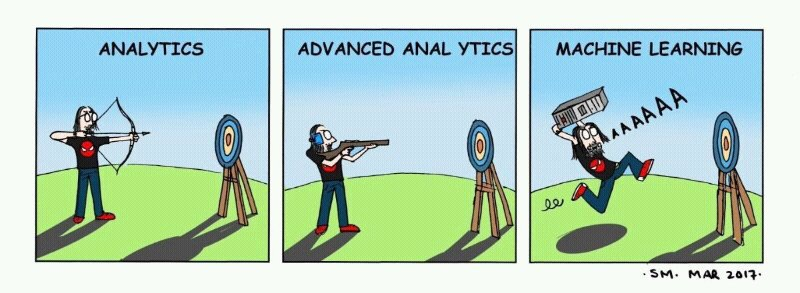
\includegraphics[width=\textwidth]{images/Chapter01_Intro/joke.jpg}
    \caption{Machine Learning.}
    \scriptsize{we could write some more}
    \label{fig: lung-breast-cancer}
    % \href{https://gco.iarc.fr}{Global cancer observatory}
\end{figure}


\section{Research Focus and Objectives}
\lipsum[2-4]
\subsection{Research question and Hypothesis}
\label{ResearchQuestion}
\lipsum[2-4]
\begin{tcolorbox}[colback=blue!5,colframe=blue!40!black,title=Hypothesis] %New Hypothesis
\textit{A hypothesis is not a question.}
\end{tcolorbox}


\subsection{Specific goals of the Research}
\label{specific-goals}
\lipsum[2-4]
\begin{enumerate}
    \item one.
    \item two.
    
\end{enumerate}

\section{Value of this Research}

\lipsum[2-4]
The remaining of this thesis is organized as follows:\\

\textbf{Chapter 1: Introduction} \\  
\lipsum[1]
 \\

\textbf{Chapter 2: Theoretical Framework }\\
\lipsum[2]
\\

\textbf{Chapter3: Research Methods} \\
\lipsum[2]\\

\textbf{Chapter4: Results} \\
\lipsum[2]\\

\textbf{Chapter 5: Conclusion} \\
\lipsum[2]\\

\textbf{Chapter 6: References} \\
\lipsum[2]

% Literature Review
\chapter{Theoretical Framework and Literature Review}
\label{chap:chap2_literature_review}
\section{Introduction}
\normalem
This Literature Review is based as always in the work by \citeauthor{Kitchenham2007} (\citeyear{Kitchenham2007}). \lipsum[4]\\

Following a SLR procedure is necessary to find a gap \parencite{Kitchenham2007}
\section{Theoretical Framework}

\begin{definition}{Machine Learning}
Some say it is not glorified statistics.
\end{definition}

\section{Literature Review}
Could it be better to use a mapping study?
\subsection{Research String}
\lipsum[5]
\subsection{Study Selection}

\chapter{Research Methods}
\label{chap:chap3_researach-methods}

\section{Introduction}

\lipsum[5]\\


\section{Problem Formulation}
In supervised learning, we aim to find a $\phi(\cdot)$ that maps an input space $\mathcal{X}$ to an output space (known as labels), $\mathcal{Y}$, as described by \eqref{eq:supervisedlearning}.

\begin{equation}
    \phi: \mathbf{\mathcal{X}} \rightarrow \mathcal{Y}    
    \label{eq:supervisedlearning}
\end{equation}

\section{Research Strategy}
Make a nice drawing of your research methodology and or strategy. This sections could be useful or not. It is up to you.

\section{Experimental Research Design}
Keep in mind that this chapter is the key to reproduce your research.\\

\lipsum[5]


\chapter{Experimental Results}
\label{chap:chap4_experimental-results}
\section{Introduction}

\lipsum[4] \\

\section{Results}
Time to present tabular information

\begin{table}[h!]
  \begin{center}
    \caption{Inbreast Transfer Learning Results on Dataset $D_{3}$}
    \label{tab:inbreast-tl-d3}
    \pgfplotstabletypeset[
      multicolumn names, % allows to have multicolumn names
      col sep=comma, % the seperator in our .csv file
      display columns/0/.style={
		column name=Algorithm, % name of first column
		column type={c},string type},  % use siunitx for formatting
      display columns/1/.style={
		column name=Metric 1,
		column type={c},string type},
	display columns/2/.style={
		column name=Metric 2,
		column type={c},string type},
	display columns/3/.style={
		column name=Metric 3,
		column type={c},string type},
      every head row/.style={
		before row={\toprule}, % have a rule at top
		after row={
% 			\si{\ampere} & \si{\volt}\\ % the units seperated by &
			\midrule} % rule under units
			},
		every last row/.style={after row=\bottomrule}, % rule at bottom
    ]{csv/results_demo.csv} % filename/path to file
    % transfer-learning-results-top5_raw_roi_not_augm.csv
  \end{center}
\end{table}


\section{Experimental Results Discussion}
Please do not leave without discussing your findings.\lipsum[5]

\chapter{Conclusion}
\section{Introduction}
\lipsum[5]

\section{Research Objectives: Summary of Findings and Conclusions}

\section{Contributions to Knowledge}
\lipsum[5]

\section{Recommendations and Future Works}
\lipsum[5]

\appendix
\chapter{Appendix}
%Images used
The appendix information goes here

\printbibliography

\end{document}
